\scanpage{19}
\diagram{\begin{tikzcd}[ampersand replacement=\&,column sep=large]
 X'=\mathbb P^1_{\mathbb Q}\arrow[r,dash]\arrow[d,"{\mu_{n\,\mathbb Q}}"'] \& \overline X'\arrow[d,dash]\\
 X=\mathbb P^1_{\mathbb Q}\arrow[r,dash]\arrow[d,dash] \& \overline X\quad 0,1,\infty,-j,-\bar j\arrow[d,dash]\\
 \mathbb Q\arrow[r,dash,"\Gamma"'] \& \overline{\mathbb Q}
\end{tikzcd}}
\[ f(z)=z^n \]
\diagram{\begin{tikzcd}[ampersand replacement=\&,column sep=small]
1\arrow[r] \& \mu_n(\overline{\mathbb Q})\arrow[r] \& \unsure{\mathcal E|\Sigma}_n\arrow[r] \& \Gamma\arrow[l,bend left=12]\arrow[r] \& 1
\end{tikzcd}}
\[ \mathcal E_n=\Gamma\mathbin{.}\mu_n(\overline{\mathbb Q}) \]

\[
\left\{\begin{aligned}
&S_0=\{0\},\quad S_1=\mu_n(\overline{\mathbb Q}),\quad S_\infty=\{\infty\}.\\
&E^+=\{z\mid z^n=-j\}\\
&E^-=\{z\mid z^n=-\bar j\}
\end{aligned}\right.
\qquad
\begin{aligned}
&\deleted{f(z)}\\
&E=\{z\mid z^{3n}=-1\deleted{\rbrace},z^n\ne-1\}
\end{aligned}
\]
\[
\begin{aligned}
R'&=\{z\mid z^n=\tfrac12\}\\
R''&=\{z\mid z^n=2\}\\
R&=\{z\mid z^n=-1\}
\end{aligned}
\qquad
\begin{aligned}
&R\\
&E\cup R=\{z\mid z^{3n}=-1\}
\end{aligned}
\]
\[
\begin{aligned}
\mathbb Q[E\cup R]&=\mathbb Q[\mu_{6n}(\overline{\mathbb Q})]\\
\rotatebox{90}{$\subset$}&\\
\mathbb Q[S_0\cup S_1\cup S_\infty]&
\end{aligned}
\]
\figure{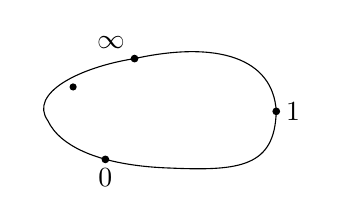
\begin{tikzpicture}[x=1cm,y=1cm]
\draw (0,0) .. controls (-.25,.35) and (.4,.68) .. (1.1,.79)
 .. controls (2.15,1.02) and (2.86,.8) .. (2.9,.12)
 .. controls (2.88,-.58) and (2.45,-.64) .. (1.55,-.60)
 .. controls (.65,-.57) and (.15,-.32) .. (0,0);
\fill (.32,.43) circle (1.3pt);
\fill (.73,-.49) circle (1.4pt) node[below] {$0$};
\fill (1.1,.79) circle (1.4pt) node[above left] {$\infty$};
\fill (2.9,.12) circle (1.4pt) node[right] {$1$};
\end{tikzpicture}}
\[
\mathbb Q[R',R'']\deleted{\unsure{R]}}=\mathbb Q[R']=\mathbb Q[\sqrt[n]{2}]
\]
\diagram{\begin{tikzcd}[ampersand replacement=\&,column sep=small]
1\arrow[r] \& \mu_{\unsure{\nu|n}}(\overline{\mathbb Q})\arrow[r] \& \Gamma'\deleted{\unsure{_n}}\arrow[r] \& (\mathbb Z/n\mathbb Z)^*\arrow[r] \& 1
\end{tikzcd}}
\[
\begin{aligned}
0,1,\infty&\mapsto0&\text{ordre }2\\
\tfrac12,2,-1&\mapsto1&\text{ordre }2\\
-j,-\bar j&\mapsto\infty&\text{ordre }3
\end{aligned}
\qquad
\begin{aligned}
\nu&=\text{ordre de }2\text{ dans }\deleted{\unsure{\mathbb Q^*}}K_n^*/K_n^{*n},\\
&\text{où }K_n=\mathbb Q(\sqrt[n]{1}).
\end{aligned}
\]
\[
g(z)=\frac{27z^2(z-1)^2}{4(z^2\unsure{-}z+1)^3}
\qquad
gf(z)=\frac{27}{4}\frac{z^{2n}(z^n-1)^2}{(z^{2n}-z^n+1)^3}
\]
\[
\lambda\frac{4}{27}=1
\]
\[
\begin{aligned}
g(z)=1&\Longleftrightarrow
\underbrace{4(z^2-z+1)^3-27z^2(z-1)^2}=0\\
&\unsure{-|=}4\big[(z+1)(z-\tfrac12)(z-2)\big]^2=4\big[(z+1)(z^2-\tfrac52+1)\big]^2\\
&\hspace{14em}=\big[(z+1)(2z^2-5+2)\big]^2
\end{aligned}
\]
% archive sheet number: 18
